\section{Photometric Calibration}
\label{sec:photometric_calibration}

We have started commissioning the full photometric calibration pipeline for
Rubin Observatory, with great success so far. For testing photometric
calibration we have obtained over 150 dithered science observations in ugriz
over the Extended Chandra Deep Field-South (ECDFS) (one of the planned LSST
deep fields), and tens more in rizy over the Euclid Deep Field South
(EDFS). All of the science data has delivered seeing of $\sim0.8$ to $\sim1.5$
arcsecond seeing.  The
validation work in this document covers the ECDFS field with more complete
filter coverage.

The precision photometric calibration software used for Rubin is the Forward
Global Calibration Method (Burke, Rykoff, et al. 2018) which was used
successfully to achieve better than 2 mmag uniformity for the Dark Energy
Survey. This software has been adapted for the LSST Science Pipelines and has
been used on Hyper Suprime Cam Special Survey Program (HSC SSP) for data
releases since DR2.

The performance on HSC data has not been as good as that on DES data due to a
number of reasons, yielding repeatability and uniformity closer to the 5 mmag
level for grizy data.  First, we have had a lot of problems with HSC
backgrounds and amp-to-amp non-linearities.  Second, the HSC survey strategy
was not well suited to self calibration due to the slow slewing of the
telescope and the long time required to change a filter, leading to lots of
isolated single-band single-night surveys.  Third, we do not have detailed
throughput scans including detector-to-detector QE variations and in-situ scans
of the significant filter variations that are required for the full forward
modeling in FGCM.

Early calibration of the ComCam data is in many ways easier than that of HSC.
First of all, we have a smaller camera (9 detectors) and thus fewer variations
to have to cross-calibrate.  Second, the camera is situated in the center and
easiest to calibrate part of the focal plane.  Third, we only have one field to
calibrate across a few nights of data so far over a limited range of airmass.
Fourth, the survey strategy (multiple bands per night dithered and repeated
with overlapping filters from night to night) is well suited to
self-calibration.  On the other hand, we do not have the CBP set up yet, so we
do not have detailed filter or detector scans available for ComCam, and are
just using the LSSTCam reference filter throughputs and average detector
throughput for the LSSTCam ITL detectors.  In addition, we do not have a flat
field screen so we have had to rely on twilight flat observations for flat fielding.

\subsection{Processing Overview}

We start with the standard ISR as documented in Section~\ref{sec:isr}. While
there are a number of challenges that we have discovered with the ITL
detectors, these are mostly near the sky level, while the testing of
photometric calibration is focused on brighter stars that are less affected by
these issues. We then apply twilight flats, which we are investigating how to
make better. At the same time, we are going to have the flat field screen and
laser and projector installed prior to the commissioning of LSSTCam, so we do
not want to spend too much time worrying about specific challenges of twilight
flats which are only necessary for ComCam.

After flat fielding we find an initial point-spread function (PSF), do a star
selection based on source and psf moments that was developed for HSC
single-frame processing, and perform an initial astrometric solution and
photometric solution (with a single zero-point per detector).  The initial
astrometric solution is used to associate star observations together prior to
global photometric calibration with FGCM.  The initial photometric solution is
used for rapid analysis and prompt processing, but is not used at all for FGCM
which relies entirely on instrumental fluxes (in units of electrons) with a
minor constraint from the reference catalog.

\subsection{Global Photometric Calibration with FGCM}

All associated stars with observations with signal-to-noise greater than 10 are
input into the FGCM solution.  In addition, reference stars from The Monster
reference catalog are associated with the stars .  Only a small fraction of the
reference stars are used in the FGCM solution, sufficient to estimate an
``absolute'' calibration (trusting that The Monster is a good absolute
reference catalog).  There is additional ongoing work with absolute calibration
with respect to the CalSpec star C26202 which is not saturated in LSST images
and is fortunately contained in ECDFS that is described below.

The FGCM model constrains the atmospheric parameters per night, as well as the
absolute throughput relative to the input scans.  The standard atmosphere is
given by MODTRAN, run at the elevation of Cerro Pachon at airmass 1.2 with an
Angstrom aerosol model.  The optics and filters are all taken from
$lsst/throughputs$ version 1.9, and the detector throughput is taken from the
ITL average of the lab scans ingested into $obs\_lsst\_data$.  Note that the
detector QEs are normalized to 1.0 at 800 nm, which is certainly
greater than the true QE at this wavelength.

\subsection{FGCM Results on the ECDFS Field}

The FGCM results presented here are based on the
\texttt{LSSTComCam/runs/DRP/20241101\_20241113/w\_2024\_46/DM-47566} DRP processing
run, specifically the 157 visits overlapping tracts
4847,4848,4849,5062,5063,5064 which are in the ECDFS field. Specifically there
are 28, 18, 38, 45, 28 visits in ugriz respectively. All QA plots are available
in the plot navigator at https://usdf-rsp.slac.stanford.edu/plot-navigator in
the collection \texttt{u/erykoff/LSSTComCam/DM-47303/test2/build2/run9}.  In this
section we focus on some of the highlights.

Note that FGCM defines a ``photometric'' observation as one that is consistent
with the forward model, including normal variations in the atmosphere, airmass,
known detector throughputs, filter curves, and additional accomodation for
aperture corrections (discussed in Burke, Rykoff et al).  With this definition
fully 92\% of the observations were deemed to be photometric by the code.

\subsubsection{Illumination Corrections}

Part of the FGCM solution is generating illumination correction maps, with a
second-order 2D Chebyshev polynomial over each detector.  Prior to LSSTCam
commissioning this will be turned into a separate calibration product generated
from dense dithered star field observations (Y1) or from the CBP (future
years). We have not yet done dithered observations with ComCam over a dense
field, only high latitude, which limits the precision.  Nevertheless we are
able to constrain reasonable illumination corrections.  The offsets from
detector to detector in the illumination correction are due to unexpected
offsets in the twilight flats that we are investigating.

\begin{figure}
  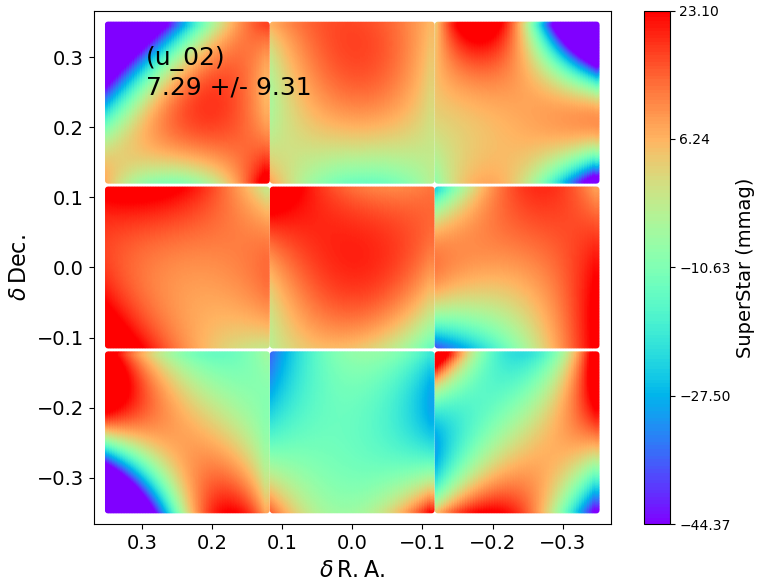
\includegraphics{photometric_calibration_figures/illumcorr_u.png}
  \caption{Illumination correction derived from FGCM for the u band.}
\end{figure}

\begin{figure}
  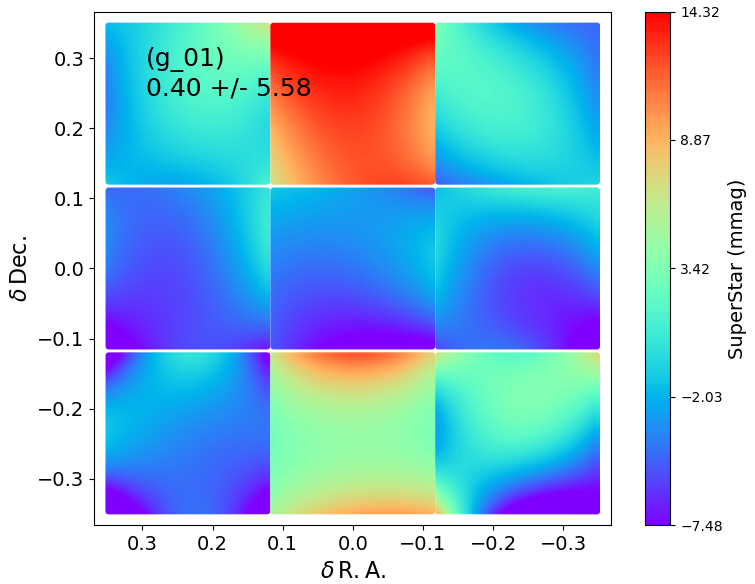
\includegraphics{photometric_calibration_figures/illumcorr_g.png}
  \caption{Illumination correction derived from FGCM for the g band.}
\end{figure}

\begin{figure}
  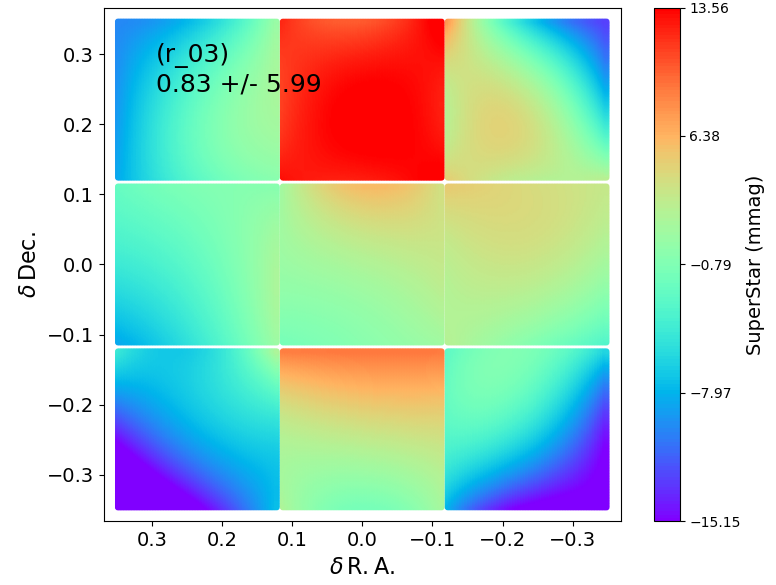
\includegraphics{photometric_calibration_figures/illumcorr_r.png}
  \caption{Illumination correction derived from FGCM for the r band.}
\end{figure}

\begin{figure}
  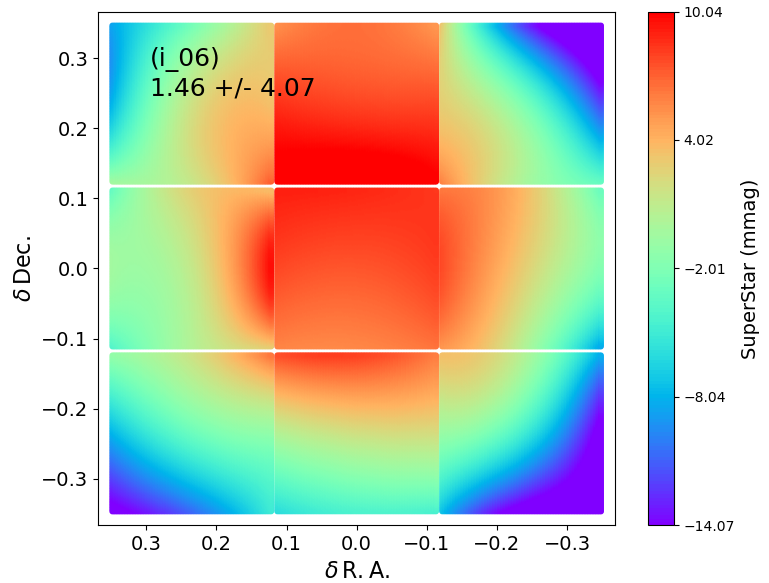
\includegraphics{photometric_calibration_figures/illumcorr_i.png}
  \caption{Illumination correction derived from FGCM for the i band.}
\end{figure}

\begin{figure}
  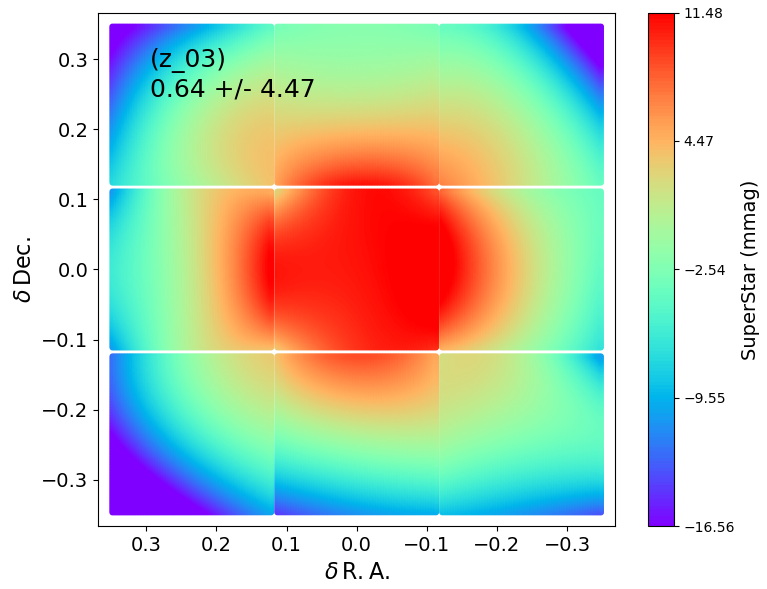
\includegraphics{photometric_calibration_figures/illumcorr_z.png}
  \caption{Illumination correction derived from FGCM for the z band.}
\end{figure}

\subsubsection{Photometric Repeatability}

The photometric repeatability after the FGCM fits was excellent. We show here
the repeatability histograms, after all chromatic corrections, for the stars
used in the fit (``all stars'').  Although 10\% of the stars are reserved,
the histograms do not yet have good statistics.  These plots are all made with
signal-to-noise greater than 100 stars (with better than 1\% photometric
errors).  Therefore the scatter is often dominated by photometric error.  The
label ``sigma\_fgcm`` is meant as an estimate of the intrinsic scatter after
subtracting off the photometric error in quadrature. The plots are split into
four panels, showing all stars, the 25\% bluest (from $g-i$ color), the 50\%
middle color, and the 25\% reddest stars. Note that the reddest stars tend to
be fainter and thus have larger photometric error. Furthermore, there are no
red stars observed in the u-band. In all cases except the u-band the intrinsic
repeatability is $1\,\mathrm{mmag}$ or better, and for the u-band it is better
than $5\,\mathrm{mmag}$, comfortably exceeding our requirements.

\begin{figure}
  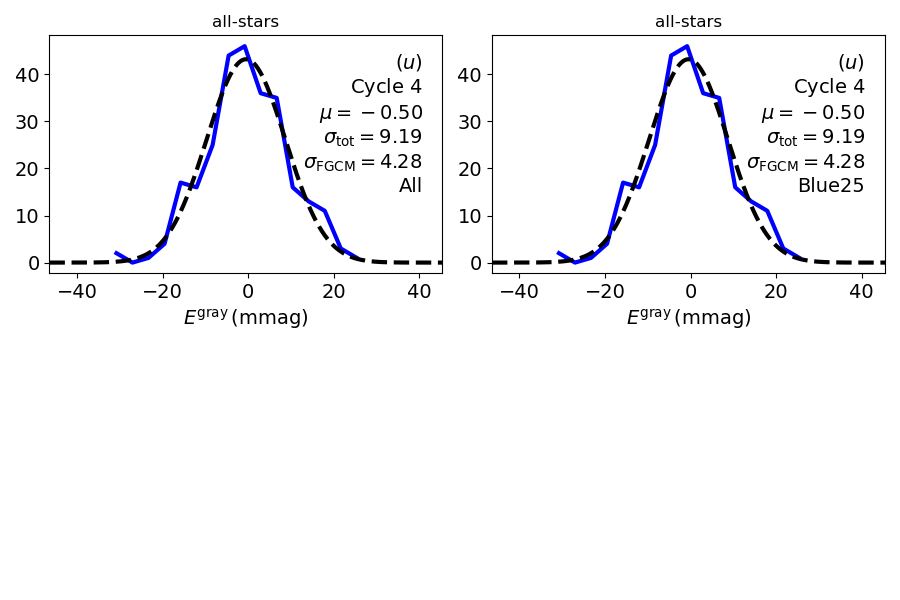
\includegraphics{photometric_calibration_figures/repeatability_u.png}
  \caption{Photometric repeatability for stars in the u band.}
\end{figure}

\begin{figure}
  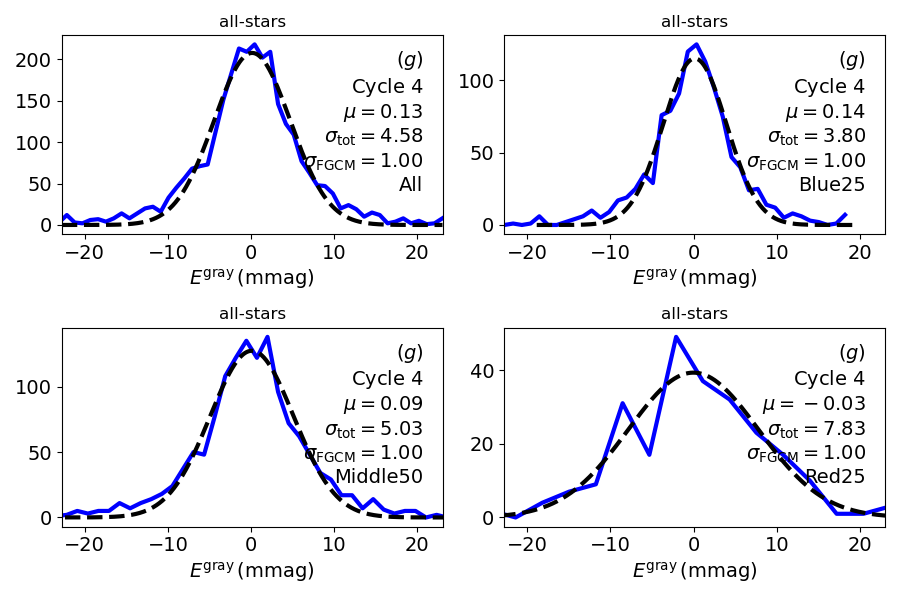
\includegraphics{photometric_calibration_figures/repeatability_g.png}
  \caption{Photometric repeatability for stars in the g band.}
\end{figure}

\begin{figure}
  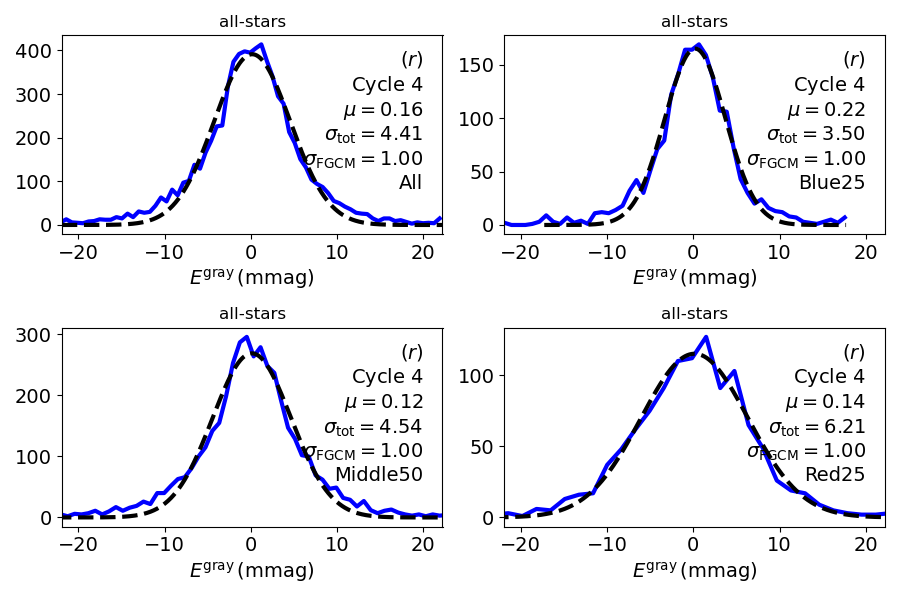
\includegraphics{photometric_calibration_figures/repeatability_r.png}
  \caption{Photometric repeatability for stars in the r band.}
\end{figure}

\begin{figure}
  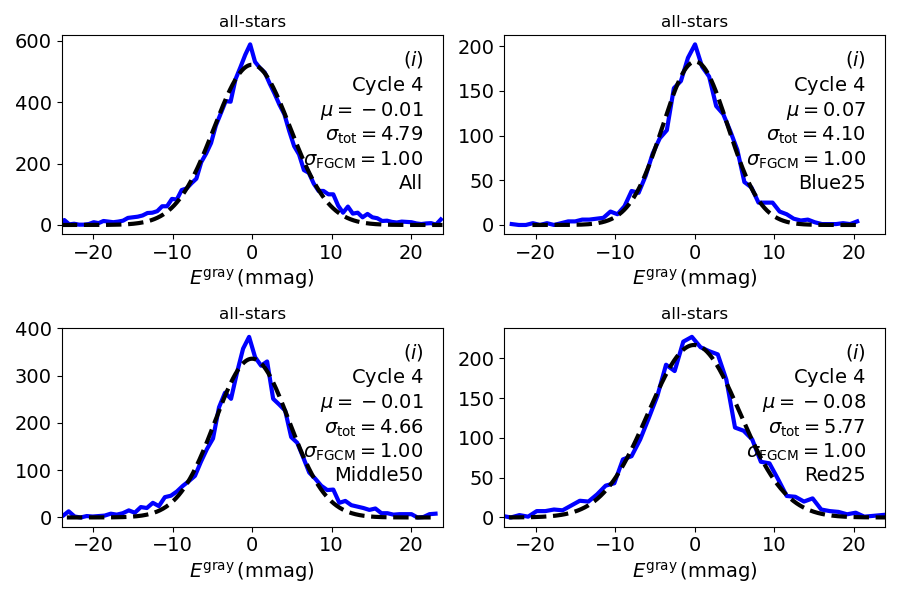
\includegraphics{photometric_calibration_figures/repeatability_i.png}
  \caption{Photometric repeatability for stars in the i band.}
\end{figure}

\begin{figure}
  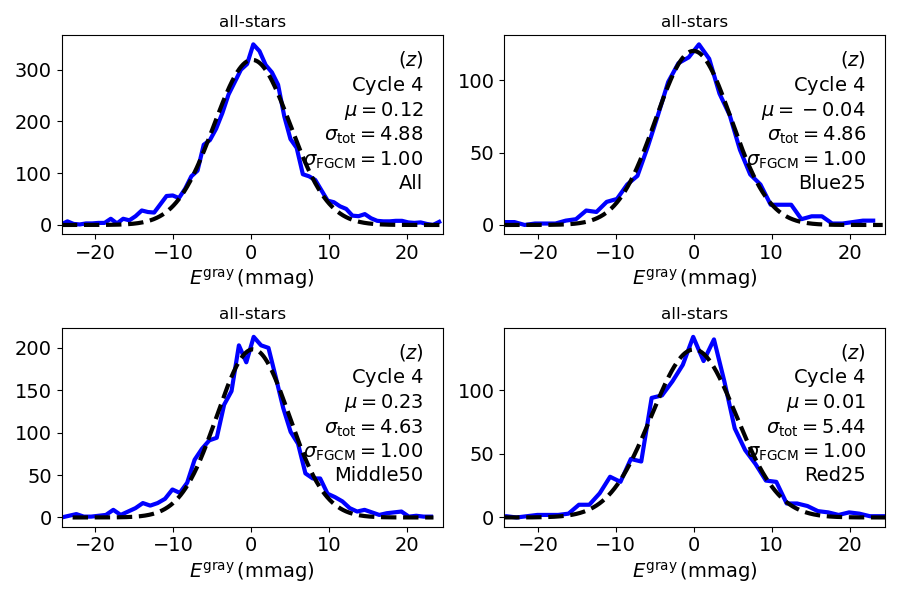
\includegraphics{photometric_calibration_figures/repeatability_z.png}
  \caption{Photometric repeatability for stars in the z band.}
\end{figure}

\subsubsection{Detector Chromaticity Fits}

In the absence of full in-situ throughput scans, we additionally constrain the
``chromaticity'' of the detectors, which is a first-order adjustment to the
slope of the peak of the throughput curve per-detector.  By doing this
adjustment in throughput space rather than color space we can preserve the
forward model approach, and additionally apply these corrections to any
SED. Note that this operation assumes that the filters are perfectly known, and
it is only the detector throughput that is varying.  This is, in general, a
valid assumption in the g band where the AR coating varies from detector to
detector causing chromatic differences in this band.

\begin{figure}
  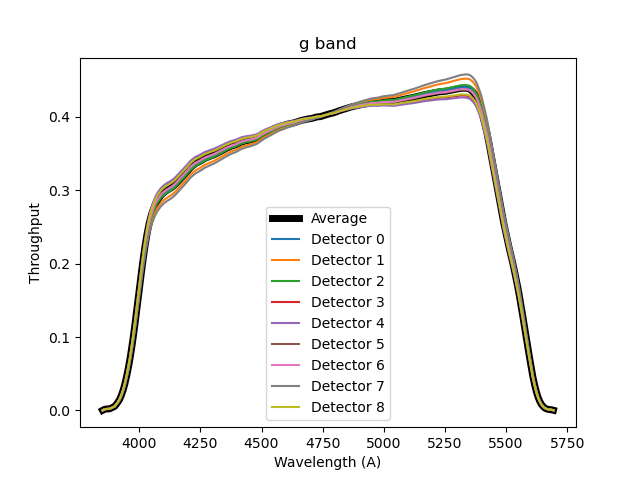
\includegraphics{photometric_calibration_figures/detector_chromaticity_g.png}
  \caption{Variation in throughput in the g band for the 9 ComCam detectors as
    derived from star colors. These are all constrained relative to the average
    ITL throughput. The CBP will be used for making this measurement
    ``correctly'', but this serves as a prediction of what variations the CBP
    scans should observe if we have it running on ComCam.}
\end{figure}

\subsubsection{Absolute Throughputs}

The FGCM fit performs a ``dead reckoning'' of the expected absolute throughput
given the telescope aperture, the effective gain, the standard atmosphere, and
the various throughputs input.  See above for the throughputs assumed.  If we
trust The Monster reference catalog for absolute calibration,
Figure~\ref{fig:absthroughputs} shows the comparison of the delivered
throughput to the predicted throughput.  In griz bands it is very close, given
that (a) we know that the peak detector QE is not 100\%; and (b) the ComCam
front lens did not have an AR coat applied, thus reducing its throughput
relative to nominal LSSTCam lenses.  In u band we are getting more throughput
than predicted.  This may be an issue with the reference catalog, or our ComCam
u-band QE is 20-30\% larger than the baseline expectation.  Given how fast the
detector QE falls off in the u-band, it would not take much to increase the
throughput by this factor.

\begin{figure}
  \label{fig:absthroughputs}
  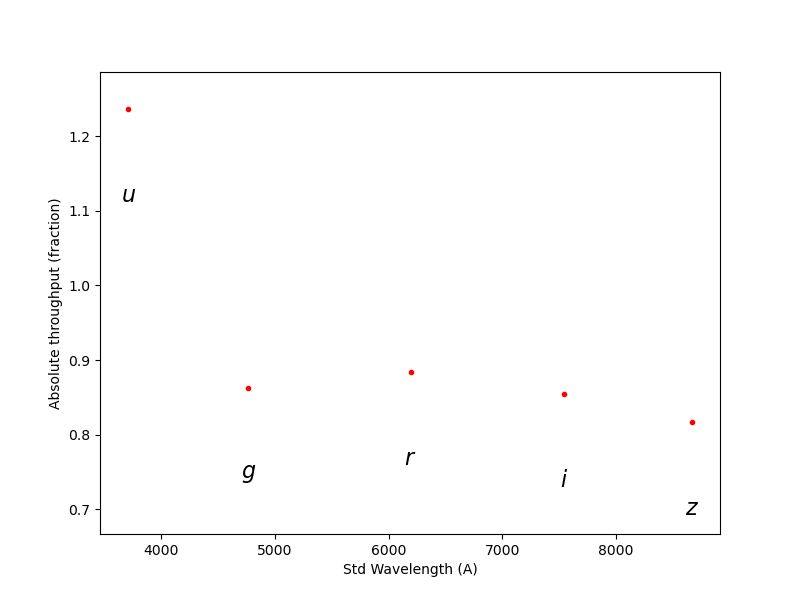
\includegraphics{photometric_calibration_figures/abs_throughput.png}
  \caption{Absolute throughput derived per band, relative to naive
    expectations.}
\end{figure}

We have additional ongoing studies of absolute throughputs using the CalSpec
standard C26202 directly.

\subsubsection{Comparison to The Monster}

Given our calibrated stars from the FGCM fit we can compare the magnitudes as a
function of color against The Monster reference catalog.  The ``lsst'' fluxes
in The Monster were derived by using stellar spectra to convert from The
Monster native DES system to the standard throughputs in lsst/throughputs
v1.9. These do not match ComCam, in particular it used a strange hybrid of
ITL/E2V for the detector throughput, which is not correct for
ComCam. Therefore, we do expect residual color terms.  Studies are ongoing on
whether these color terms are expected given the differences between the ComCam
throughput and the predicted LSST throughput.  Further validation will be
possible if we get CBP scans prior to the removal of ComCam.

\begin{figure}
  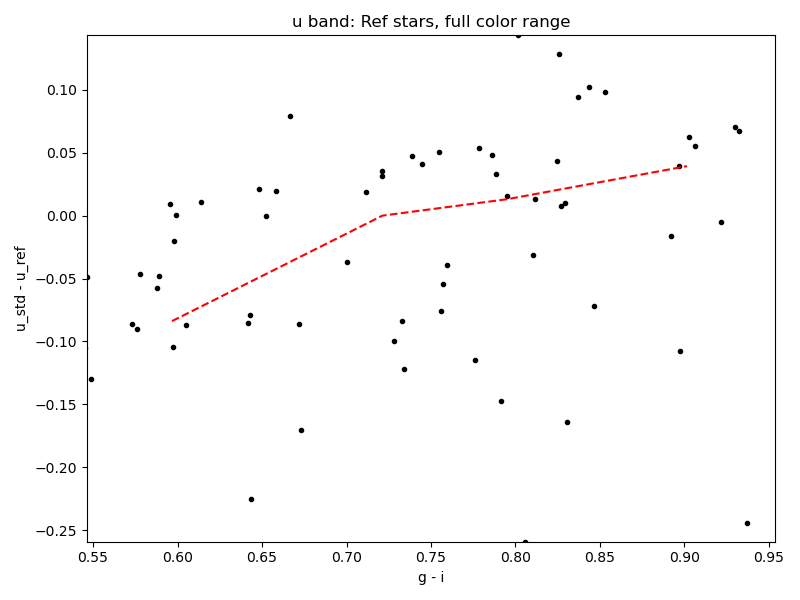
\includegraphics{photometric_calibration_figures/reference_residuals_u.png}
  \caption{Residuals between FGCM standardized magnitudes and The Monster
    predicted LSST magnitudes for the u band as a function of $g-i$, assuming
    The Monster has the correct absolute throughput.}
\end{figure}

\begin{figure}
  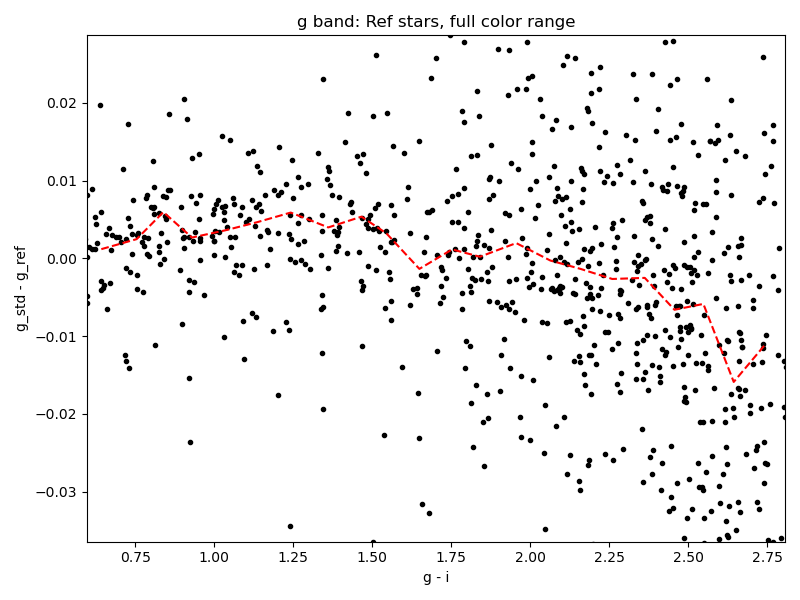
\includegraphics{photometric_calibration_figures/reference_residuals_g.png}
  \caption{Residuals between FGCM standardized magnitudes and The Monster
    predicted LSST magnitudes for the g band as a function of $g-i$, assuming
    The Monster has the correct absolute throughput.}
\end{figure}

\begin{figure}
  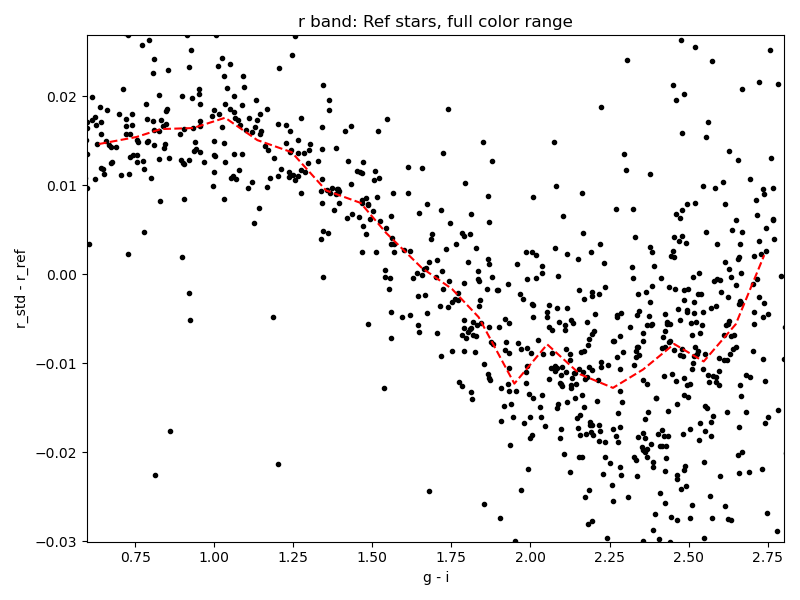
\includegraphics{photometric_calibration_figures/reference_residuals_r.png}
  \caption{Residuals between FGCM standardized magnitudes and The Monster
    predicted LSST magnitudes for the r band as a function of $g-i$, assuming
    The Monster has the correct absolute throughput.}
\end{figure}

\begin{figure}
  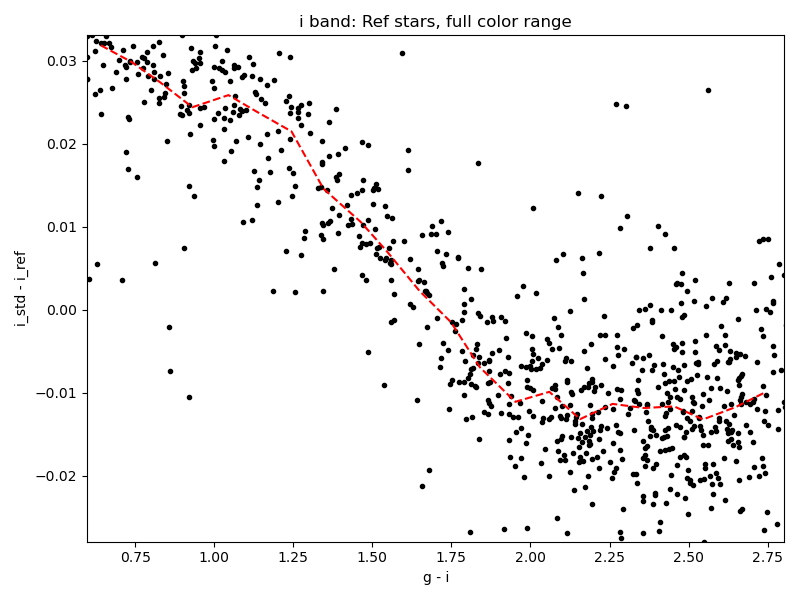
\includegraphics{photometric_calibration_figures/reference_residuals_i.png}
  \caption{Residuals between FGCM standardized magnitudes and The Monster
    predicted LSST magnitudes for the i band as a function of $g-i$, assuming
    The Monster has the correct absolute throughput.}
\end{figure}

\begin{figure}
  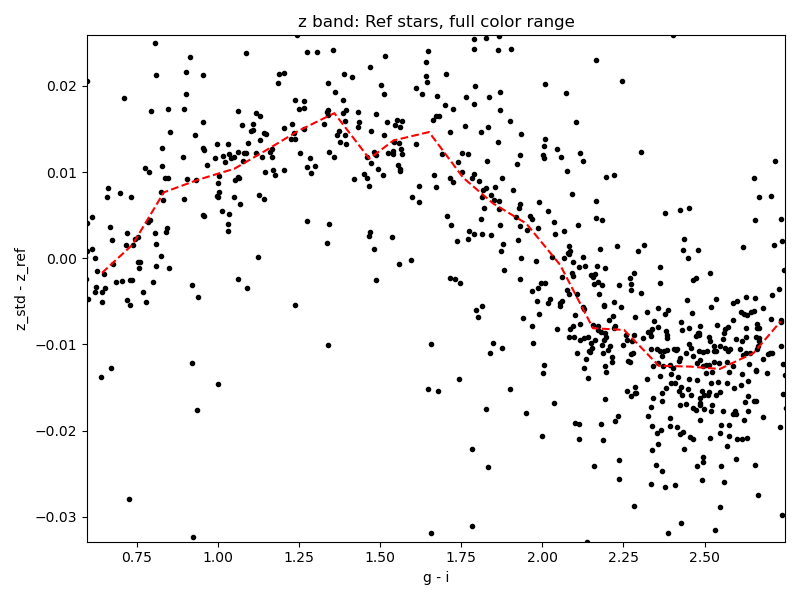
\includegraphics{photometric_calibration_figures/reference_residuals_z.png}
  \caption{Residuals between FGCM standardized magnitudes and The Monster
    predicted LSST magnitudes for the z band as a function of $g-i$, assuming
    The Monster has the correct absolute throughput.}
\end{figure}

\subsubsection{Background Oversubtraction}

As a side-effect in the calibration, FGCM tests local background
oversubtraction by looking at the statistical difference between two large
aperture magnitudes.  If the background were perfectly measured then the
difference in magnitude will just be a measure of the wings of the PSF (a local
portion of the growth curve) which should be self-similar for all star fluxes.
Instead, we generally see a downturn consistent with a constant background
offset.  This background oversubtraction has been seen in DES, HSC, and
ComCamSim data at similar levels with different photometric pipelines.  It is
worse in the redder bands.  It seems to be caused by the far wings of stars (in
DES all stars and galaxies brighter than 17th magnitude in i contribute), as
well as possibly due to faint undetected sources.  This same background
oversubtraction effect is seen in the ComCam images.  Further investigations
are being done by the low-surface-brightness science unit.

\begin{figure}
  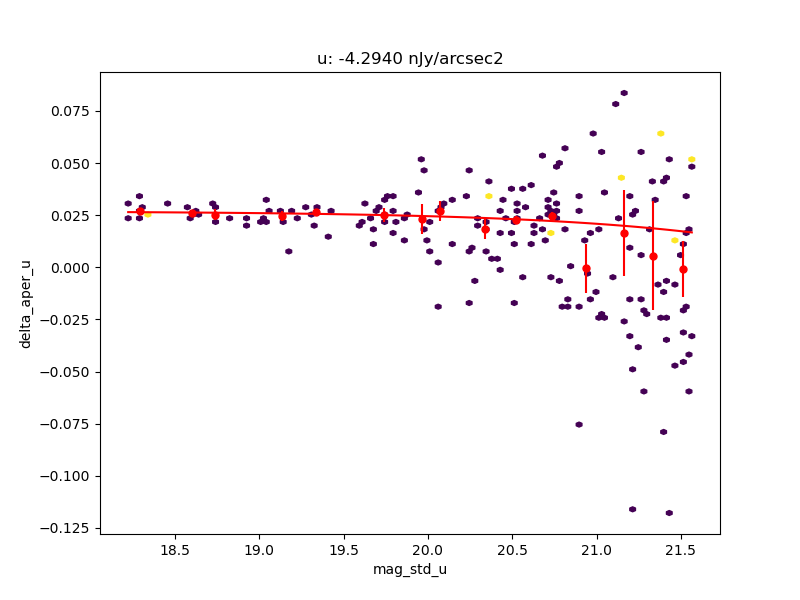
\includegraphics{photometric_calibration_figures/background_oversubtraction_u.png}
  \caption{Estimate of the background oversubtraction using delta magnitudes
    from large apertures in the u band.  The amount of curvature is a measure
    of the oversubtraction; this should be flat as a function of star magnitude
    if the background were measured correctly on average.}
\end{figure}

\begin{figure}
  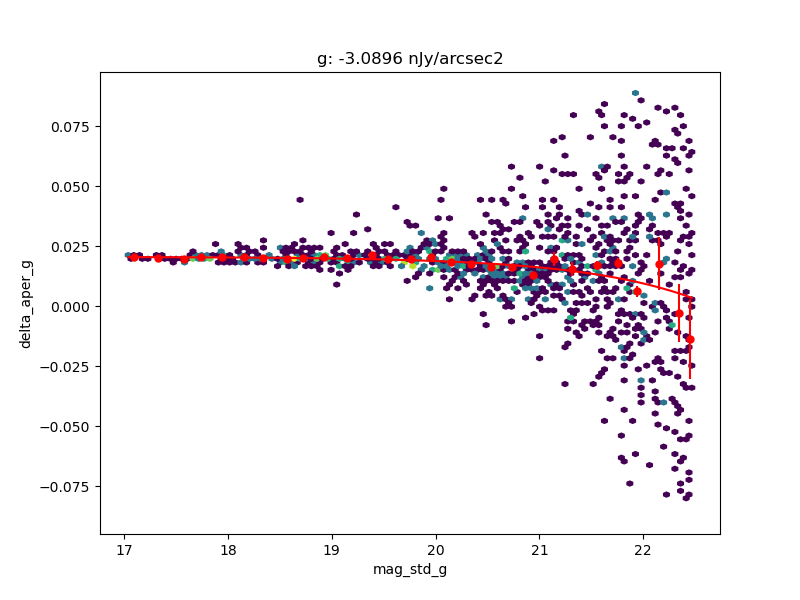
\includegraphics{photometric_calibration_figures/background_oversubtraction_g.png}
  \caption{Estimate of the background oversubtraction using delta magnitudes
    from large apertures in the g band.  The amount of curvature is a measure
    of the oversubtraction; this should be flat as a function of star magnitude
    if the background were measured correctly on average.}
\end{figure}

\begin{figure}
  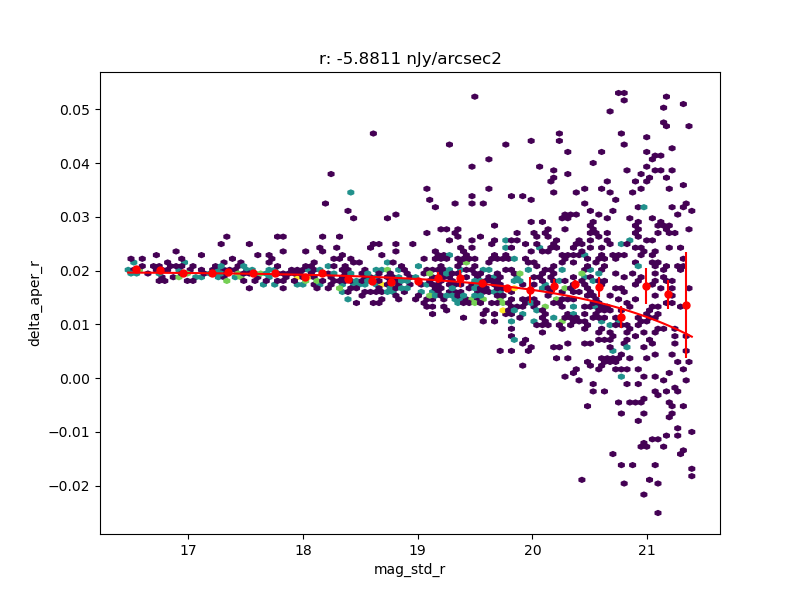
\includegraphics{photometric_calibration_figures/background_oversubtraction_r.png}
  \caption{Estimate of the background oversubtraction using delta magnitudes
    from large apertures in the r band.  The amount of curvature is a measure
    of the oversubtraction; this should be flat as a function of star magnitude
    if the background were measured correctly on average.}
\end{figure}

\begin{figure}
  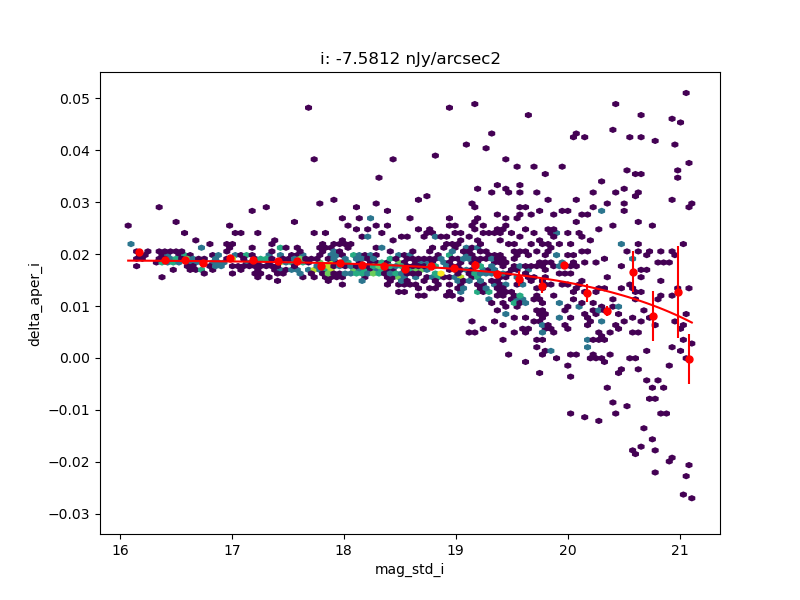
\includegraphics{photometric_calibration_figures/background_oversubtraction_i.png}
  \caption{Estimate of the background oversubtraction using delta magnitudes
    from large apertures in the i band.  The amount of curvature is a measure
    of the oversubtraction; this should be flat as a function of star magnitude
    if the background were measured correctly on average.}
\end{figure}

\begin{figure}
  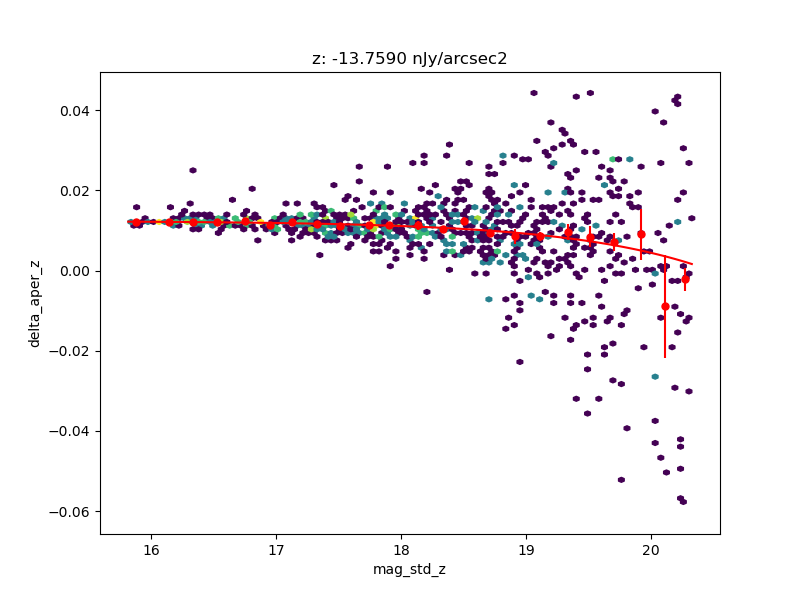
\includegraphics{photometric_calibration_figures/background_oversubtraction_z.png}
  \caption{Estimate of the background oversubtraction using delta magnitudes
    from large apertures in the z band.  The amount of curvature is a measure
    of the oversubtraction; this should be flat as a function of star magnitude
    if the background were measured correctly on average.}
\end{figure}

\subsection{Next Steps}

The following additional data will need be taken to advance from our current
knowledge:

\begin{enumerate}
  \item{g band observations in the EDFS field, when the g filter is put back
    into ComCam for the upcoming dark time.}
  \item{Dithered observations in as many bands as possible over a field with
    much larger stellar density for better illumination corrections.}
  \item{More contiguous dithered survey data in (at least) gri.}
\end{enumerate}

The particular emphasis on g band in these requests is that by default FGCM
will use the $g-i$ color for internal QA, which is a very useful color to split
on.  There are no facilities in the code for doing quality calibrations on
multiple disconnected fields with different band coverage, as this is not the
normal case for survey observations.  We could run different fields separately
with different configs, but this is not preferred.  Thus, gri coverage over the
fields of interest for DRP processing is the ``easiest'' path that will yield
the best results and be most consistent with the LSST survey.
